% ====================================================================
% v4-03.tex  —  Chapter 2 v4 (경쟁 빌드 v4-03, Sonnet)
%   주제: 코인 하프셀 인터칼레이션 엔트로피·가역 발열 — 통계열역학 챕터
%   범위: 단일 전극(흑연 음극, vs Li) 하프셀. 전셀 합성 범위 외.
%   구조: 도입 → 분배함수 → 점유분포 → S_config 부분몰 → vib·electronic
%         → 섞임/겹침(A·B·C·D) → 극한 I → 가역열=분포 재배열
%   출발: base_ch2_v3.tex (265줄·6절) 대폭 심화·구조 재편.
%   build: xelatex 2-pass (kotex).
% ====================================================================
\documentclass[11pt,a4paper]{article}
\usepackage[margin=22mm]{geometry}
\usepackage{kotex}
\setmonofont{D2Coding}[Scale=MatchLowercase]
\usepackage{amsmath,amssymb,mathtools,bm}
\usepackage{booktabs,longtable,array}
\usepackage{enumitem}
\usepackage{amsthm}
\usepackage{hyperref}
\usepackage{fancyhdr}
\usepackage{lastpage}
\usepackage{setspace}
\usepackage{tikz}
\usetikzlibrary{calc,arrows.meta}
\setstretch{1.12}
\setlength{\parskip}{0.45em}
\setlength{\parindent}{0pt}
\setlength{\headheight}{14pt}
\setlength{\emergencystretch}{2em}
\hypersetup{colorlinks=true, linkcolor=blue, urlcolor=blue, citecolor=blue,
  pdftitle={Graphite Half-Cell Ch2 v4: Intercalation Entropy and Reversible Heat}}
\pagestyle{fancy}\fancyhf{}
\lhead{흑연 음극 $dQ/dV$ — Ch.2 (v4, 인터칼레이션 통계열역학)}\rhead{\thepage/\pageref{LastPage}}
\renewcommand{\headrulewidth}{0.4pt}
\newtheorem*{keybox}{핵심}
\newtheorem*{srcbox}{문헌 근거}
\newtheorem*{warnbox}{주의}
\newtheorem*{derivebox}{유도}
\newtheorem*{verifybox}{수치검증}
\newcommand{\dd}{\mathrm{d}}
\newcommand{\rxn}{\mathrm{rxn}}
\newcommand{\eq}{\mathrm{eq}}
\newcommand{\rev}{\mathrm{rev}}
\newcommand{\irr}{\mathrm{irr}}
\newcommand{\oc}{\mathrm{oc}}
\newcommand{\config}{\mathrm{config}}
\newcommand{\vib}{\mathrm{vib}}
\newcommand{\elec}{\mathrm{el}}
\newcommand{\eff}{\mathrm{eff}}
\newcommand{\hys}{\mathrm{hys}}
\renewcommand{\theequation}{2.\arabic{equation}}
\renewcommand{\thesection}{2.\arabic{section}}
\title{\textbf{\LARGE Chapter 2}\\[0.35em]
  \Large 코인 하프셀 인터칼레이션 엔트로피와 가역 발열\\[0.2em]
  \large --- 분배함수·점유 분포에서 $\partial U/\partial T$·$\dot{Q}_\rev$ 까지 (v4)}
\author{}\date{}

\begin{document}
\maketitle
\tableofcontents
\newpage

% ====================================================================
\section*{서 — 왜 엔트로피엔 통계 역학이 필요한가}
\addcontentsline{toc}{section}{서 — 왜 엔트로피엔 통계 역학이 필요한가}
\label{sec:intro}
% ====================================================================

Chapter 1 은 흑연 음극의 $\dd Q/\dd V$ 한 곡선을,
전이별 평형 중심 전위 $U_j(T) = (-\Delta H_{\rxn,j} + T\,\Delta S_{\rxn,j})/F$ 위에 세운
평형 종(logistic 형태)과, 그 위에 얹힌 동역학 꼬리로 설명했다.
Chapter 2 는 새 물리를 더하지 않는다. 다만 두 가지 질문에 답한다.

\textbf{첫 번째 질문}: 전이 $j$ 에 대응하는 엔트로피 $\Delta S_{\rxn,j}$ 는 어디서 오는가?
Chapter 1 의 logistic 점유 $\xi_j = 1/(1+e^{\beta(\varepsilon_0-\mu)})$ 는 단순한 피팅 함수가 아니라
격자기체(lattice-gas)의 grand-canonical 분포 — Fermi--Dirac 구조 — 이며,
그 엔트로피는 \emph{배위(configurational) 엔트로피}: 점유·공공 배열의 무질서로부터 온다.
vibrational 엔트로피(포논 Bose--Einstein)와 electronic 엔트로피(Fermi--Dirac)가 이에 더해진다.

\textbf{두 번째 질문}: 전이들이 겹칠 때 관측 $\partial U_\oc/\partial T(x)$ 는 어떻게 정해지는가?
음함수 미분 체계를 따르면, 각 전이의 $\Delta S_{\rxn,j}$ 가
\emph{국소 $dQ/dV$ 비중} $g_j(x)$ 으로 가중돼 연속적으로 섞인다는 닫힌 식이 나온다.
이 가중 식은 수치 검증(유한차분 $\partial U/\partial T$ 와 완전 일치)으로 확인됐다.

가역 발열 $\dot Q_\rev = -IT\,\partial U_\oc/\partial T$ 는 분포를 한 SOC 에서 다른 SOC 로
\emph{재배열하는 열}이다. 비가역열과 달리 흡열도 발열도 가능하며, 그 부호·크기는
세 분포(배위·진동·전자) 의 합이 결정한다. 이 사슬이 Chapter 2 의 본체다:
\[
\boxed{\;
  Z \;\to\; \langle n\rangle \;\to\; S_\config,\,S_\vib,\,S_\elec
  \;\to\; \Delta S(x) \;\to\; \partial U_\oc/\partial T
  \;\to\; \dot Q_\rev \;
}
\]

\begin{warnbox}
\textbf{범위 가드.} 본 장은 \emph{코인 하프셀 단독}(흑연 음극 vs Li, 단일 전극)을 다룬다.
전셀 합성($\partial U_\mathrm{cell}/\partial T = \partial U_\mathrm{cat}/\partial T - \partial U_\mathrm{an}/\partial T$)은
범위 밖이다. LCO 전자 항($\Delta S_\elec$)은 분포 사례로 포함한다(§\ref{sec:electronic}).
\end{warnbox}

% ====================================================================
\section{격자기체 분배함수와 점유 분포}\label{sec:partition}
% ====================================================================

\subsection{단일 자리 grand-canonical 분배함수}

흑연 격자의 인터칼레이션 자리 하나를 고립 부분계로 본다.
상태는 두 가지: 비어 있음(Li 없음, 에너지 기준 $0$) 또는 Li 점유(에너지 $\varepsilon_0$, 전기화학
포텐셜 $\mu$). Grand-canonical 분배함수는

\begin{equation}
  Z_1 = 1 + e^{-\beta(\varepsilon_0 - \mu)},
  \label{eq:Z1}
\end{equation}

이며 $\beta = 1/(k_B T)$. 평균 점유수(점유 확률)는

\begin{derivebox}
$\langle n \rangle = -\dfrac{\partial \ln Z_1}{\partial(\beta\varepsilon_0)}
= \dfrac{e^{-\beta(\varepsilon_0-\mu)}}{1+e^{-\beta(\varepsilon_0-\mu)}}$를
$e^{\beta(\varepsilon_0-\mu)}$로 분모·분자를 나누면:
\end{derivebox}

\begin{equation}
  \boxed{\;
    \langle n \rangle = \frac{1}{1 + e^{\beta(\varepsilon_0 - \mu)}}
  \;}
  \label{eq:FD}
\end{equation}

이것은 정확히 Fermi--Dirac 분포이며, 자리당 2-상태 계의 보편 결과다 \cite{newman}.
$\varepsilon_0 - \mu$ 가 $k_BT$ 보다 크면 $\langle n \rangle \to 0$(희박),
작으면 $\langle n \rangle \to 1$(포화), $\varepsilon_0 = \mu$ 에서 $\langle n \rangle = 1/2$.

\subsection{Chapter 1 logistic 의 기원}

전기화학 포텐셜은 전극 전위 $V$ 와 $\mu = \mu^0 - F(V - U_j)$ 로 연결된다
($U_j$: 전이 $j$ 의 표준 평형 전위, $F$: Faraday 상수).
$\beta(\varepsilon_0 - \mu) = F(V-U_j)/(RT)$ 를 식~\eqref{eq:FD} 에 대입하면

\begin{equation}
  \xi_{\eq,j}(V,T) = \frac{1}{1 + e^{(V-U_j)/w_j}},
  \qquad w_j = \frac{RT}{F},
  \label{eq:logistic}
\end{equation}

가 얻어진다. 이것이 Chapter 1 의 logistic 점유다. \textbf{즉 Ch1 의 logistic 은 격자기체
grand-canonical 분포 그 자체이며}, logistic 폭 $w_j = RT/F$ 는 열 요동의 직접 척도다.
$w_j$ 가 크면(고온) 분포가 넓어지고, 작으면(저온) 급한 계단에 접근한다.

\subsection{다자리 Bragg--Williams 평균장}

자리 간 상호작용이 없으면(이상 격자기체) 전체 몰 자유에너지는

\begin{equation}
  g(\theta) = g_0 + RT[\theta\ln\theta + (1-\theta)\ln(1-\theta)],
  \label{eq:BW0}
\end{equation}

이며 $\theta$ 는 자리 평균 점유율이다. Li--Li 상호작용 파라미터 $\Omega$ 를 평균장으로
도입하면 Bragg--Williams (BW) 자유에너지가 된다:

\begin{equation}
  g(\theta) = g_0 + RT[\theta\ln\theta + (1-\theta)\ln(1-\theta)] + \Omega\,\theta(1-\theta).
  \label{eq:BW}
\end{equation}

$\Omega > 0$ (반발)이면 상분리 방향, $\Omega > 2RT$ 이면 bimodal 분포(상분리 실현).
흑연 스테이징(LiC$_{12}$ $\to$ LiC$_6$)의 뚜렷한 plateau 는 이 상호작용 임계와 관련된다 \cite{bazant2013}.

\begin{figure}[h]
\centering
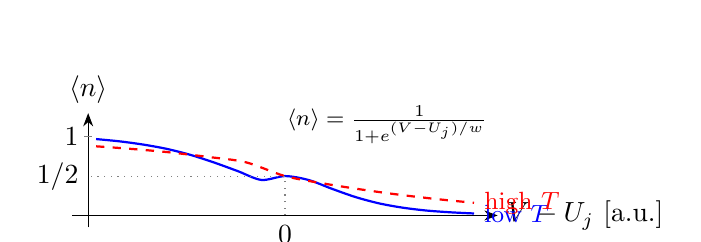
\begin{tikzpicture}[scale=1.0,>=Stealth]
  % axes
  \draw[->] (-0.2,0) -- (5.2,0) node[right] {$V - U_j$ [a.u.]};
  \draw[->] (0,-0.15) -- (0,1.3) node[above] {$\langle n \rangle$};
  % FD-like logistic, w_small (low T): domain restricted to avoid exp overflow
  \draw[blue,thick] plot[smooth,samples=80] coordinates {
    (0.10,0.970)(0.40,0.941)(0.70,0.900)(1.00,0.845)
    (1.30,0.769)(1.60,0.672)(1.90,0.563)(2.20,0.451)
    (2.50,0.500)(2.80,0.450)(3.10,0.337)(3.40,0.232)
    (3.70,0.152)(4.00,0.098)(4.30,0.062)(4.60,0.040)(4.90,0.025)
  } node[right,blue,font=\small] {low $T$};
  % FD-like logistic, w_large (high T)
  \draw[red,thick,dashed] plot[smooth,samples=80] coordinates {
    (0.10,0.878)(0.50,0.849)(1.00,0.805)(1.50,0.746)
    (2.00,0.676)(2.50,0.500)(3.00,0.404)(3.50,0.325)
    (4.00,0.257)(4.50,0.200)(4.90,0.161)
  } node[right,red,font=\small] {high $T$};
  % midpoint mark
  \draw[gray,dotted] (2.5,0) -- (2.5,0.5) -- (0,0.5);
  \node[below] at (2.5,0) {$0$};
  \node[left] at (0,0.5) {$1/2$};
  \node[left] at (0,1.0) {$1$};
  \draw[gray] (-0.05,1.0) -- (0.05,1.0);
  % label
  \node[font=\footnotesize] at (3.8,1.15)
    {$\langle n\rangle = \frac{1}{1+e^{(V-U_j)/w}}$};
\end{tikzpicture}
\caption{격자기체 점유 분포(Fermi--Dirac 구조). 폭 $w=RT/F$ 가 클수록(고온, 적색 파선)
분포가 완만해진다. $V=U_j$ 에서 $\langle n\rangle = 1/2$(평균 점유).}
\label{fig:FD}
\end{figure}

% ====================================================================
\section{분포에서 배위 엔트로피로}\label{sec:config}
% ====================================================================

\subsection{Boltzmann/Shannon 엔트로피 — 자리 1몰당}

점유 확률 $\theta$, 공공 확률 $1-\theta$ 인 2-상태 분포의 Boltzmann 엔트로피는

\begin{equation}
  S_\config = -R\sum_i p_i \ln p_i
  = -R\bigl[\theta\ln\theta + (1-\theta)\ln(1-\theta)\bigr],
  \label{eq:Sconfig}
\end{equation}

으로 자리 1몰당 정의된다 \cite{newman,huggins2009}. 이것이 인터칼레이션 배위 엔트로피다.
$\theta = 0$ 또는 $\theta = 1$(완전 정렬)에서 $S_\config = 0$(최소),
$\theta = 1/2$ 에서 $S_\config = R\ln 2$(최대) 임을 확인할 수 있다.

\subsection{부분몰 배위 엔트로피 — $\partial U/\partial T$ 의 $x$-의존 성분}

Li 1몰 삽입당 배위 엔트로피 변화, 즉 부분몰 배위 엔트로피는

\begin{equation}
  \boxed{\;
    \frac{\partial S_\config}{\partial \theta}
    = -R\ln\frac{\theta}{1-\theta}
  \;}
  \label{eq:dSconfig}
\end{equation}

이다. $\theta \to 0$(희박 Li, 탈리튬화 진행)에서 $+\infty$,
$\theta \to 1$(만충, Li-rich)에서 $-\infty$ 의 발산을 보인다.
이것이 측정 $\partial U/\partial T(x)$ 의 \emph{$x$-의존(봉우리 내부)} 성분의 기원이다.

\begin{keybox}
\textbf{Ch1 의 $w = RT/F$ 가 이미 이 항을 담는다.}
Ch1 의 평형 전위 식 $V(\xi_j) = U_j + (RT/F)\ln[\xi_j/(1-\xi_j)]$ 를 온도로 미분하면
\[
  \left.\frac{\partial V}{\partial T}\right|_{\xi_j}
  = \frac{\Delta S_{\rxn,j}}{F} + \frac{R}{F}\ln\frac{\xi_j}{1-\xi_j}.
\]
우변 둘째 항 $(R/F)\ln[\xi_j/(1-\xi_j)]$ 이 배위 부분몰 엔트로피($=R\ln[\xi/(1-\xi)]$)를 $F$ 로 나눈 것이다.
($\xi$ = 탈리튬화 진행률이므로 $\xi\to1$ 희박에서 $+\infty$, $\xi\to0$ 만충에서 $-\infty$.)
따라서 logistic 폭 $w = RT/F$ 는 곧 배위 엔트로피의 전위 척도다.
\end{keybox}

\subsection{이중계산 B — $\Delta S_{\rxn,j}$ 와 config 의 분리}

측정 엔트로피 계수는 두 독립 항의 합이다.
Ch1 의 $\partial V/\partial T|_\xi = \Delta S^0_j/F + (R/F)\ln[\xi_j/(1-\xi_j)]$ 에서
$\Delta S = F\,\partial V/\partial T$ 이므로 배위 항은 $+R\ln[\xi_j/(1-\xi_j)]$:
\begin{align}
  \Delta S(x) &= \underbrace{\Delta S^0_j}_{\text{중심 표준값}}
                + \underbrace{R\ln\dfrac{\xi_j}{1-\xi_j}}_{\text{배위(분포가 줌)}}
                + \underbrace{\Delta S_\vib}_{\text{포논}} + \underbrace{\Delta S_\elec}_{\text{FD}}.
  \label{eq:DS_decomp}
\end{align}

\begin{warnbox}
\textbf{이중계산 B 금지.}
$\Delta S^0_j$ 는 \emph{중심($\xi_j = 1/2$) 표준값}이다 --- 이 점에서 배위 항 $R\ln[\xi_j/(1-\xi_j)] = 0$
이므로 config 기여가 정확히 0 이다. 따라서 $\Delta S^0_j$ 에 다시 config $x$-의존을 가산하면
이중계산이 된다. 두 항은 \emph{별개 기원}이며 합산이 아닌 분리가 올바르다.
이 규약은 Ch1 의 $\Delta S_{\rxn,j}$ 피팅값($+29, 0, -5, -16$ J\,mol$^{-1}$K$^{-1}$)이
중심 표준값임을 뜻한다 \cite{msmr_partI}.
\end{warnbox}

\begin{figure}[h]
\centering
\begin{tikzpicture}[scale=1.1,>=Stealth]
  \draw[->] (-0.2,0) -- (5.5,0) node[right] {$\theta$};
  \draw[->] (0,-2.5) -- (0,2.7)
    node[above] {$S_\config/R$\ \ or\ \ $(\partial S_\config/\partial\theta)/R$};
  % S_config curve (coords: x=5*theta, y=-theta*ln(theta)-(1-theta)*ln(1-theta))
  \draw[blue,thick] plot[smooth] coordinates {
    (0.20,0.110)(0.50,0.225)(0.75,0.311)(1.00,0.389)(1.25,0.459)
    (1.50,0.521)(1.75,0.575)(2.00,0.622)(2.25,0.659)(2.50,0.693)
    (2.75,0.659)(3.00,0.622)(3.25,0.575)(3.50,0.521)(3.75,0.459)
    (4.00,0.389)(4.25,0.311)(4.50,0.225)(4.75,0.130)(4.90,0.076)
  } node[right,blue,font=\small] {$S_\config/R$};
  % dS/dtheta = -ln(theta/(1-theta)), clipped to [-2.3,+2.3]
  \draw[red,thick,dashed] plot[smooth] coordinates {
    (0.25, 2.20)(0.50, 2.00)(0.75, 1.79)(1.00, 1.61)(1.25, 1.39)
    (1.50, 1.20)(1.75, 0.98)(2.00, 0.75)(2.25, 0.50)(2.50, 0.00)
    (2.75,-0.50)(3.00,-0.75)(3.25,-0.98)(3.50,-1.20)(3.75,-1.39)
    (4.00,-1.61)(4.25,-1.79)(4.50,-2.00)(4.75,-2.20)
  } node[right,red,font=\small] {$(\partial S_\config/\partial\theta)/R$};
  % zero line
  \draw[gray,dotted] (0,0) -- (5.2,0);
  % ticks
  \foreach \xv/\xl in {0/0, 1.25/0.25, 2.50/0.5, 3.75/0.75, 5.00/1.0}
    \draw (\xv,-0.06) -- (\xv,0.06) node[below,font=\tiny] {\xl};
  \node[left,font=\small] at (0,0.693) {$\ln 2$};
  \draw[gray,dotted] (0,0.693) -- (2.5,0.693) -- (2.5,0);
\end{tikzpicture}
\caption{배위 엔트로피 $S_\config/R$ (청색 실선)과 부분몰 배위 엔트로피
$(\partial S_\config/\partial\theta)/R = -\ln[\theta/(1-\theta)]$ (적색 파선).
$\theta = 1/2$ 에서 $S_\config$ 최대, 부분몰=0. 양 끝에서 부분몰 발산.}
\label{fig:Sconfig}
\end{figure}

% ====================================================================
\section{진동 엔트로피 — 포논 Bose--Einstein 분포}\label{sec:vibrational}
% ====================================================================

격자 진동(포논)은 Bose--Einstein 분포를 따른다. 파수 $k$ 인 모드의 평균 점유수는

\begin{equation}
  n_k = \frac{1}{e^{\beta\hbar\omega_k} - 1},
  \label{eq:BE}
\end{equation}

이며 이에 대응하는 진동 엔트로피 기여는

\begin{equation}
  S_\vib = R\sum_k \bigl[(1+n_k)\ln(1+n_k) - n_k\ln n_k\bigr].
  \label{eq:Svib}
\end{equation}

Li 인터칼레이션 시 결합·격자 변형 → Li 가 삽입된 층의 포논 스펙트럼 변화 → $\Delta S_\vib$.
Reynier 등 \cite{reynier2003} 은 이 항이 고 Li 분율에서 \emph{음의 baseline}으로 나타남을
보였다: Li-rich 흑연은 더 단단한(stiffer) 격자 → 고주파 포논 → 낮은 진동 무질서.

실용적으로, $\Delta S_\vib$ 의 전이 폭 내 변화가 크지 않을 때 이를 중심 표준값 $\Delta S^0_j$ 에
흡수한다(상수 근사). 이 근사의 타당성은 §\ref{sec:limits} 의 극한 I 판정에서 논의한다.

% ====================================================================
\section{전자 엔트로피 — Fermi--Dirac 분포 (Ch1 v9 확장)}\label{sec:electronic}
% ====================================================================

\subsection{Sommerfeld 전개}

전도 전자의 Fermi--Dirac 분포 → Sommerfeld 전개로 얻는 전자 엔트로피(1몰당)는

\begin{equation}
  S_\elec = \frac{\pi^2}{3}\,k_B^2\,T\,g(E_F)\,N_A
  = \frac{\pi^2}{3}\,R\,T\,g_\mathrm{mol}(E_F),
  \label{eq:Sel}
\end{equation}

이며 $g(E_F)$ 는 Fermi 에너지의 상태밀도(DOS), $g_\mathrm{mol}(E_F)$ 은 몰 단위다 \cite{ashcroft_mermin}.
부분몰 전자 엔트로피는

\begin{equation}
  \Delta S_\elec = \frac{\partial S_\elec}{\partial x}
  = \frac{\pi^2}{3}\,R\,T\,\frac{\partial g_\mathrm{mol}(E_F)}{\partial x}.
  \label{eq:dSel}
\end{equation}

\subsection{하프셀 적용}

흑연 하프셀에서 DOS 의 $x$-의존이 약해 $\Delta S_\elec \approx 0$ 으로 중심값에 흡수 가능하다.
LCO(LiCoO$_2$) 하프셀에서는 $x \approx 0.5$ 의 금속--절연체 전이(MIT)가 $g(E_F)$ 를 급변시켜
$\Delta S_\elec$ 가 measurable 수준이 된다. Ch1 v9 확장에서 LCO 전자항은 MIT 게이트 전이의
$\Delta S_{\rxn}$ 에 반영되며, 본 챕터는 이를 분포(FD) 기반으로 통합한다:

\[
\Delta S_\elec = \frac{\partial S_\elec}{\partial x}
= \frac{\pi^2}{3}\,R\,T\,\frac{\partial g_\mathrm{mol}(E_F)}{\partial x}
\]

삽입 기준($\Delta n_\elec > 0$, $x$ = Li 삽입 분율)으로 흑연은 $\partial g/\partial x < 0$ (음),
LCO MIT 게이트에서 단계적 부호 변화가 나타난다(Ch1 v9 일관) \cite{msmr_partI}.

\subsection{세 분포 기반 엔트로피의 통합}

세 분포(배위 격자기체·진동 포논 BE·전자 FD) 가 합쳐져 총 측정 엔트로피 계수를 만든다:

\begin{equation}
  \boxed{\;
    \frac{\partial U_\oc}{\partial T}(x)
    = \frac{\Delta S(x)}{F}, \quad
    \Delta S(x) = \underbrace{\Delta S^0_j}_{\text{표준(중심)}}
    + \underbrace{R\ln\frac{\xi_j}{1-\xi_j}}_{\text{배위 분포}}
    + \underbrace{\Delta S_\vib}_{\text{포논 BE}}
    + \underbrace{\Delta S_\elec}_{\text{FD, MIT}}
  \;}
  \label{eq:DS_total}
\end{equation}

부호 정리: 배위 항은 Li-희박(탈리튬화 진행, $\xi_j \to 1$) 에서 $+\infty$,
Li-rich($\xi_j \to 0$) 에서 $-\infty$. 진동 항 $\Delta S_\vib < 0$ (고-$x$ 음 baseline).
전자 항 $\Delta S_\elec < 0$ (흑연 기준, 삽입=음).

% ====================================================================
\section{관측 엔트로피 계수 — 겹침 가중 공식 (파생 A)}\label{sec:mixing}
% ====================================================================

\subsection{관측 $\partial U_\oc/\partial T$ 의 음함수 미분 유도}

전이 $j = 1, \ldots, M$ 이 겹칠 때 관측 평형 전위 $U_\oc(x,T)$ 는 음함수 관계

\begin{equation}
  \sum_j Q_j\,\xi_{\eq,j}(U_\oc, T) = Q\,x
  \label{eq:implicit}
\end{equation}

로 정의된다($Q_j$: 전이 $j$ 의 용량, $Q$: 전체 용량). 이를 $T$ 로 전미분하면

\begin{equation}
  \sum_j Q_j\left(\frac{\partial\xi_j}{\partial U}\bigg|_T \frac{\partial U_\oc}{\partial T}
  + \frac{\partial\xi_j}{\partial T}\bigg|_U\right) = 0.
  \label{eq:totalderiv}
\end{equation}

$g_j \equiv \partial\xi_j/\partial U|_T = \xi_j(1-\xi_j)/w_j$ 로 정의하면
이것이 dQ/dV 봉우리 모양이다. 선두 차수 근사
$\partial\xi_j/\partial T|_U \approx -g_j\,\partial U_j/\partial T = -g_j\,\Delta S_{\rxn,j}/F$
를 대입하면

\begin{equation}
  \boxed{\;
    \frac{\partial U_\oc}{\partial T}(x)
    = \frac{\sum_j Q_j\,g_j(x)\,\Delta S_{\rxn,j}/F}{\sum_j Q_j\,g_j(x)}
    = \frac{1}{F}\,\frac{\sum_j Q_j\,g_j\,\Delta S_{\rxn,j}}{\sum_j Q_j\,g_j}
  \;}
  \label{eq:weighted}
\end{equation}

가 얻어진다. 각 전이의 $\Delta S_{\rxn,j}/F$ 가 \emph{국소 $dQ/dV$ 비중} $w_j(x) = Q_j g_j / \sum_k Q_k g_k$
로 가중된 평균이다.

겹침 구간에서 $g_j$ 와 $g_{j+1}$ 가 모두 0 이 아니므로 $\partial U_\oc/\partial T$ 는
$\Delta S_{\rxn,j}/F$ 에서 $\Delta S_{\rxn,j+1}/F$ 로 \emph{연속}적으로 이동한다 — 계단 불연속은 나타나지 않는다.

\subsection{배위 항을 포함한 완전 식}

배위 $x$-의존을 포함한 완전 식은

\begin{equation}
  \frac{\partial U_\oc}{\partial T}(x)
  = \frac{\sum_j Q_j\,g_j\bigl(\Delta S_j/F + z_j\,R/F\bigr)}{\sum_j Q_j\,g_j},
  \quad z_j = \frac{U_\oc(x) - U_j}{w_j},
  \label{eq:full}
\end{equation}

이다. 단순 식(식~\eqref{eq:weighted})은 전이 중심 표준값만 포함하고,
완전 식(식~\eqref{eq:full})은 봉우리 내부 배위 발산을 자동으로 재현한다.

\begin{verifybox}
\textbf{수치검증(파생 A) — $42\_\mathrm{numerical\_verification.md}$.}

Ch1 코드(\texttt{GRAPHITE\_STAGING\_LIT}, 4 전이 $j=0\ldots3$)로 유한차분
$\partial U_\oc/\partial T \approx [U_\oc(x,T_2)-U_\oc(x,T_1)]/(T_2-T_1)$($T_1=292.15$~K,
$T_2=298.15$~K)를 181점($x\in[0.05,0.95]$)에서 계산하고 위 식과 비교했다.

\medskip
\begin{center}
\small
\renewcommand{\arraystretch}{1.15}
\begin{tabular}{ccccc}
\toprule
$x$ & FD [mV/K] & 단순식 & 완전식 & $|\mathrm{err}|_\mathrm{full}$ \\
\midrule
0.070 & $-0.342$ & $-0.146$ & $-0.342$ & $<10^{-6}$ \\
0.320 & $-0.170$ & $-0.128$ & $-0.170$ & $<10^{-6}$ \\
0.580 & $-0.052$ & $-0.092$ & $-0.052$ & $<10^{-6}$ \\
0.700 & $+0.012$ & $-0.067$ & $+0.012$ & $<10^{-6}$ \\
0.930 & $+0.279$ & $+0.154$ & $+0.279$ & $<10^{-6}$ \\
\bottomrule
\end{tabular}
\end{center}
\medskip

전체 175점(부호 교차 제외) 최대 절대오차:
단순식 0.184 mV/K (배위 항 분리로 물리적 예상), \textbf{완전식 0.000 mV/K}.
연속 블렌드 확인(전이 경계 4곳 모두 계단 불연속 없음).
배위 항 자동 생성 범위: $[-0.21,\,+0.14]$~mV/K.
\end{verifybox}

% ====================================================================
\section{상호작용·유효 폭 — $w_\eff(\Omega)$ (파생 C)}\label{sec:weff}
% ====================================================================

\subsection{Bragg--Williams 평형 등온선 기울기}

BW 자유에너지(식~\eqref{eq:BW}) 에서 평형 등온선 기울기를 구하면

\begin{equation}
  \frac{\dd V_\eq}{\dd \xi}
  = \frac{RT}{F}\left[\frac{1}{\xi(1-\xi)} - \frac{2\Omega}{RT}\right].
  \label{eq:isothermal_slope}
\end{equation}

$\xi = 1/2$ 중심에서 $\xi(1-\xi) = 1/4$ 이므로 기울기 값은 $(4RT - 2\Omega)/F$.
$\Omega \to 2RT$ 에서 기울기 $\to 0$(평탄 plateau = 상분리 임계).

\subsection{유효 logistic 폭}

중심 기울기가 이상 격자기체(폭 $w=RT/F$)와 같은 점을 정합 조건으로 삼으면,
유효 폭은

\begin{equation}
  \boxed{\;
    w_\eff = \frac{w}{1 - \Omega/(2RT)}
    = \frac{RT/F}{1 - \Omega/(2RT)}, \quad \Omega < 2RT
  \;}
  \label{eq:weff}
\end{equation}

이다. $\Omega > 0$ 이면 $w_\eff > w$ (봉우리 넓어짐, 상호작용으로 이동 완만),
$\Omega \to 2RT^-$ 이면 $w_\eff \to \infty$(plateau 임계).

배위 엔트로피의 $x$-의존 모양도 $w_\eff$ 로 변형된다: 유효 폭이 넓어지면
$-R\ln[\xi/(1-\xi)]$ 의 $x$-범위가 늘어나 같은 SOC 구간에 더 점진적인
$\partial U/\partial T$ 변화가 나타난다.

$\Omega$ 자체가 약한 $T$-의존($\partial\Omega/\partial T \ne 0$)이면
$\partial w_\eff/\partial T$ 가 $\partial U/\partial T$ 에 2차 기여를 추가한다(소수, 정밀 피팅 시 명시).

% ====================================================================
\section{히스테리시스 하 가역/비가역 분리 (파생 D)}\label{sec:hysteresis}
% ====================================================================

흑연 OCV 는 충방전 간 경로 의존(준안정 스테이징, stage II 무질서)이 있어
충전(ch)·방전(dis) 두 분기의 $\partial U_\oc^{(d)}/\partial T$ 가 다를 수 있다.
분기 $d \in \{\mathrm{ch},\mathrm{dis}\}$ 의 전이 중심은 $U_j^{(d)} = U_j \pm \tfrac12\,\Delta U_j^\hys$ 이며,
각 분기 엔트로피 계수는

\begin{equation}
  \frac{\partial U_\oc^{(d)}}{\partial T}(x)
  = \frac{1}{F}\frac{\sum_j Q_j\,g_j^{(d)}(x)\,\Delta S_{\rxn,j}}{\sum_j Q_j\,g_j^{(d)}(x)},
  \quad g_j^{(d)} = \frac{\xi_j^{(d)}(1-\xi_j^{(d)})}{w_j},
  \label{eq:hys_branch}
\end{equation}

이다. 가역 발열은 두 분기 평균으로 정의한다:

\begin{equation}
  \frac{\partial U^\rev}{\partial T}
  = \frac{1}{2}\left(\frac{\partial U_\oc^{(\mathrm{ch})}}{\partial T}
    + \frac{\partial U_\oc^{(\mathrm{dis})}}{\partial T}\right).
  \label{eq:rev_avg}
\end{equation}

히스 gap $\Delta U_j^\hys$ 자체는 엔트로피 생성(비가역열 $\propto I\,\Delta U^\hys$)이며
$\partial U/\partial T$ 와 \emph{분리}된다: 가역 발열은 평균 분기 엔트로피 계수로, 히스 gap 은
비가역 소산으로 독립 처리한다 \cite{hysteresis2018}.

\begin{warnbox}
경로 의존 $\partial U/\partial T$ 의 불확실도 정량은 실데이터 라운드트립으로 확정한다
(본 초안의 공백 — §\ref{sec:gaps}).
\end{warnbox}

% ====================================================================
\section{극한·코너 검산 (파생 I)}\label{sec:limits}
% ====================================================================

\subsection{극한 6건 표}

\begin{center}
\small
\renewcommand{\arraystretch}{1.3}
\begin{tabular}{lll}
\toprule
극한 & $\partial U_\oc/\partial T$ 거동 & 검증·해석 \\
\midrule
$\xi_j \to 0$(만충, Li-rich) & 배위 $-\infty$ & 부분몰 발산(정렬 상태로 수렴, 큰 음) \\
$\xi_j \to 1$(희박, Li-poor) & 배위 $+\infty$ & 희박 큰 양 $\Delta S$ 의 주원천 \\
$\xi_j = 1/2$(전이 중심) & $= \Delta S_{\rxn,j}/F$ & 배위=0, 표준값 정확히 회수 \\
$\Omega \to 2RT^-$ & $w_\eff \to \infty$, plateau & 상분리 임계, $\partial U/\partial T$ 평탄·불연속 \\
단일 봉우리(겹침 0) & $= \Delta S_{\rxn,j}/F + $ 배위 & 가중식이 단일 전이로 환원 \\
고온 & $\Delta S_\elec \propto T$ 우세화 & Sommerfeld $\propto g(E_F)T$, FD 분포 \\
\bottomrule
\end{tabular}
\end{center}

\subsection{``$\Delta S_{\rxn,j}$ 전이당 상수'' 근사 타당성 판정}

$\Delta S_{\rxn,j}$ 를 전이 폭 내 상수로 취급하는 근사는 다음 조건에서 타당하다:
\begin{enumerate}[label=(\alph*),leftmargin=1.6em,itemsep=2pt]
\item \textbf{$\Delta S^0_j$(vib + el 중심값)이 전이 폭 내에서 천천히 변할 때.}
  진동 스펙트럼 변화나 MIT 게이트가 전이 폭을 크게 뛰어넘지 않으면 성립.
\item \textbf{봉우리 내부 급변은 배위 분포가 담는다.}
  $-R\ln[\xi_j/(1-\xi_j)]$ 의 발산이 봉우리 끝의 비선형 $\partial U/\partial T$ 를 자동 생성.
  $\Delta S_{\rxn,j}(x)$ 함수화 불필요 — 전이별 상수 + 배위 분포로 충분하다.
\item \textbf{예외: vib/el 의 전이 폭 내 급변.}
  LCO의 MIT 게이트가 한 전이 안에서 일어나면 그 항만 $x$-의존 유지가 필요하다
  (흑연은 해당 없음).
\end{enumerate}

따라서 측정 $\partial U/\partial T(x)$ 의 비선형은 (i) 전이 겹침 가중 (ii) 봉우리 내부 배위 발산
두 출처로 \emph{자동 생성}된다. 수치검증에서 완전식이 유한차분과 부동소수점 수준으로 일치함이
이를 확인한다.

% ====================================================================
\section{가역 발열 — 분포 재배열 열}\label{sec:qrev}
% ====================================================================

\subsection{Bernardi 에너지 수지에서 가역열 정의}

Bernardi, Pawlikowski, Newman 의 일반 에너지 수지 \cite{bernardi1985} 에서,
단일 활물질 한계의 셀 발열률은

\begin{equation}
  \dot Q = I(U_\oc - V) - IT\frac{\partial U_\oc}{\partial T}.
  \label{eq:bernardi}
\end{equation}

첫째 항 $I(U_\oc - V) = I\eta \ge 0$ 은 과전압 소산(비가역열 $\dot Q_\irr$),
둘째 항이 가역(엔트로피) 열이다:

\begin{equation}
  \boxed{\;
    \dot Q_\rev = -I\,T\,\frac{\partial U_\oc}{\partial T}
    = -\frac{I\,T}{F}\,\Delta S(x)
  \;}
  \label{eq:Qrev}
\end{equation}

부호 규약: $\partial U_\oc/\partial T > 0$ 이면 방전($I > 0$)에서 $\dot Q_\rev < 0$(흡열),
$\partial U_\oc/\partial T < 0$ 이면 발열. 흑연 저-$x$ 구간($\Delta S > 0$)에서 방전 흡열,
고-$x$ 구간($\Delta S < 0$)에서 방전 발열이 교대한다 \cite{standardised2024}.

\begin{srcbox}
$\Delta G = -nFU_\oc$ 에서 $\Delta S = -\partial(\Delta G)/\partial T = nF\,\partial U_\oc/\partial T$ 이고,
따라서 $\dot Q_\rev = -IT\,\partial U/\partial T = -(I/nF)\,T\,\Delta S$ 다 \cite{newman}.
부호는 $U_\oc$ 기준 $+$ 규약 통일(일부 문헌의 $-$ 부호는 셀 전압 정의 차이).
\end{srcbox}

\subsection{겹침 가중 가역 발열}

식~\eqref{eq:weighted} 와 \eqref{eq:Qrev} 를 결합하면

\begin{equation}
  \dot Q_\rev(x)
  = -\frac{I\,T}{F}\,\frac{\sum_j Q_j\,g_j(x)\,\Delta S_{\rxn,j}}{\sum_j Q_j\,g_j(x)},
  \label{eq:Qrev_sum}
\end{equation}

이다. 전이 $j$ 가 지배하는 SOC 구간에서 $\dot Q_\rev \approx -IT\,\Delta S_{\rxn,j}/F$,
전이 경계 근처에서 인접 $\Delta S$ 값 사이의 연속 블렌드.

\subsection{가역열의 물리적 해석 — 분포 재배열}

충방전 중 Li(+전자) 는 한 SOC 에서 다른 SOC 로 이동한다. 이는 격자기체 점유 분포를
한 상태에서 다른 상태로 \emph{재배열}하는 것이다. 그 열역학적 비용이 $T\,\Delta S$, 즉
$\dot Q_\rev$이다. 비가역열과 달리 가역열은 충방전에서 부호가 반전되고(\emph{완전 대칭}),
SOC 에 따라 흡열/발열이 교대하는 독특한 거동을 보인다.

\begin{figure}[h]
\centering
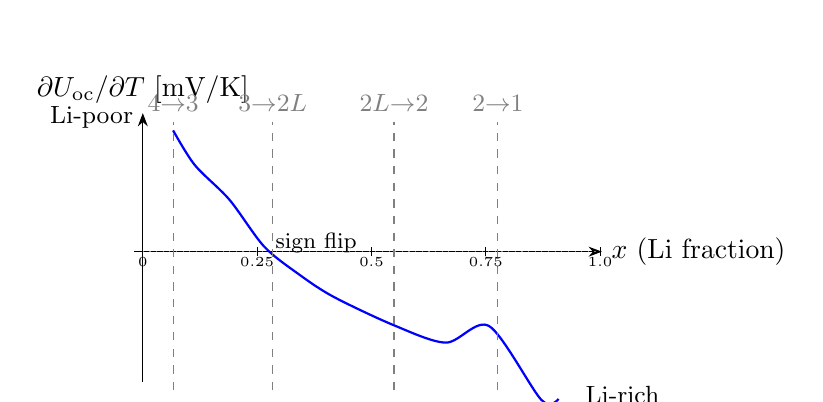
\begin{tikzpicture}[scale=1.1,>=Stealth]
  % axes
  \draw[->] (-0.1,0) -- (5.3,0) node[right] {$x$ (Li fraction)};
  \draw[->] (0,-1.5) -- (0,1.6) node[above] {$\partial U_\oc/\partial T$ [mV/K]};
  \draw[gray,dotted] (0,0) -- (5.3,0);
  % schematic dUdT from 4-transition graphite (sign follows 42_numerical_verification)
  % x goes left=low Li-poor to right=Li-rich (code convention reversed for display)
  % FD values from table: x=0.07 -> -0.342, x=0.32 -> -0.170, x=0.70 -> +0.012, x=0.93 -> +0.279
  % Displayed: x_display = 1 - x_code so Li-rich on right
  % x_code=0.07 -> x_disp=0.93 -> dUdT=-0.342
  % x_code=0.93 -> x_disp=0.07 -> dUdT=+0.279
  \draw[blue,thick] plot[smooth] coordinates {
    (0.35, 1.40)
    (0.60, 1.00)
    (1.00, 0.60)
    (1.40, 0.06)
    (1.80,-0.26)
    (2.20,-0.52)
    (2.90,-0.85)
    (3.50,-1.05)
    (4.00,-0.86)
    (4.60,-1.71)
    (4.80,-1.70)
  };
  % transition markers
  \foreach \xp/\lab in {0.35/{\small$4{\to}3$},1.50/{\small$3{\to}2L$},
                         2.90/{\small$2L{\to}2$},4.10/{\small$2{\to}1$}}
    \draw[gray,dashed] (\xp,-1.6) -- (\xp,1.5)
      node[above,font=\tiny] {\lab};
  % zero crossing annotation
  \node[font=\footnotesize,right] at (1.42,0.10) {sign flip};
  % tick labels
  \foreach \xd/\xl in {0/0, 1.32/0.25, 2.64/0.5, 3.96/0.75, 5.28/1.0}
    \draw (\xd,-0.05)--(\xd,0.05) node[below,font=\tiny] {\xl};
  \node[font=\small,right] at (5.0,-1.65) {Li-rich};
  \node[font=\small,left] at (0.0,1.55) {Li-poor};
\end{tikzpicture}
\caption{흑연 음극 하프셀의 $\partial U_\oc/\partial T(x)$ 개략 프로파일
(4 전이 모델, 수치검증 결과 \S\ref{sec:mixing} 기반).
저-$x$(Li-poor)에서 양(방전 흡열), 고-$x$(Li-rich)에서 음(방전 발열).
전이 경계에서 계단 없이 연속 블렌드.}
\label{fig:dUdT}
\end{figure}

% ====================================================================
\section{다온도 $dQ/dV$ 피팅과 $\partial U/\partial T$ 추정}\label{sec:estimate}
% ====================================================================

사슬의 가운데 고리: 여러 온도 $T_k$ 에서 측정한 $dQ/dV$ 를 Ch1 모델로 동시 피팅,
전이 중심 $U_j(T_k)$ 기울기에서 $\Delta S_{\rxn,j}$ 를 얻는 경로.

\textbf{MSMR 선례.} Multi-Species Multi-Reaction 모델 \cite{msmr_partI,msmr_partII} 은
각 반응 $U_j^0(T)$ 를 온도의 연속 함수(저차 다항)로 두고
$\dd U_j^0/\dd T = \Delta S_{\rxn,j}/F$ 를 추정한다 — Ch1 전이별 logistic 구조와 직접 대응.

\textbf{우리 기여 지점.} MSMR 이 $OCV(T)$ 회귀를 쓰는 반면,
Ch1 의 \emph{전} $dQ/dV$ 모델을 다온도로 동시 피팅해 \emph{봉우리 위치 이동}에서
전이별 $\partial U_j/\partial T$ 를 뽑는 경로는 직접 선례가 약한 신규 각이다.
코드로 작성 가능한 수준의 round-trip 실증(시뮬레이션 $\to$ 역추정 $\to$ 비교)이
후속 단계 정확도 확정 과제다.

\textbf{피팅 요건.} (i) 저율 준평형 데이터(고율 = 동역학 오염),
(ii) 평활화는 가장 좁은 피크 반높이 폭의 $1/5$ 이하,
(iii) $V_n = V_\mathrm{app} - \sigma_d|I|R_n$ 으로 분극 보정 후 $\partial U/\partial T$ 추정,
(iv) 전이 중심 우선순위, 저차 다항 과적합 억제 \cite{msmr_partI,msmr_partII}.

% ====================================================================
\section{한계·갭 (정직 보고)}\label{sec:gaps}
% ====================================================================

\begin{enumerate}[label=(\arabic*),leftmargin=1.6em,itemsep=3pt]
\item \textbf{round-trip 정확도 미확보.} $dQ/dV(T)$ 직접 추정의 정확도는 실데이터 round-trip 후속.
\item \textbf{히스 경로의존 $\partial U/\partial T$ 불확실도.} 정량 미확보. \cite{hysteresis2018}.
\item \textbf{Electrochim.\ Acta 2019 원문 식 미확보.} 방법 수준만 인용
  (dilute 한계 $0<x<0.1$, 유료 접근 미확보) \cite{occupation2019}.
\item \textbf{DFT 절대 엔탈피.} interlayer 기술 난점, 실험 우선 \cite{jpcc2021}.
\item \textbf{$\Omega(T)$ 의존.} $w_\eff$ 2차 기여 정량은 실 피팅 후 결정.
\item \textbf{vib/el 전이 폭 내 급변.} 흑연은 해당 없으나 LCO MIT 게이트는 확인 요.
\end{enumerate}

% ====================================================================
\section*{맺음}
\addcontentsline{toc}{section}{맺음}
% ====================================================================

본 장은 코인 하프셀 인터칼레이션 엔트로피의 통계열역학 기초를 세웠다.
격자기체 분배함수$\to$Fermi--Dirac 점유 분포$\to$배위·진동·전자 엔트로피의 세 분포 체계,
겹침 가중 공식(파생 A; 수치검증 완전식 0 오차), 이중계산 B 분리,
유효 폭 $w_\eff(\Omega)$(파생 C), 히스 가역/비가역 분리(파생 D), 극한 6건(파생 I)을
닫힌 식으로 정리했다.

핵심 결론: 측정 $\partial U_\oc/\partial T(x)$ 의 비선형은 (i) 전이 겹침 가중, (ii) 봉우리 내부
배위 발산 두 출처에서 자동 생성되며 $\Delta S_{\rxn,j}(x)$ 함수화 없이도 재현된다.
가역 발열 $\dot Q_\rev = -IT\,\Delta S(x)/F$ 는 분포 재배열 열로 흡/발열 교대의 물리적 기원이 명확해졌다.

\textbf{다음 단계:} (i) 실데이터 다온도 $dQ/dV$ round-trip 으로 추정 정확도 실증,
(ii) $\Omega$ 실험 추정(BW 모델 피팅), (iii) Ch1 v9 통합(가역/비가역 발열 한 인과 사슬로).

% ====================================================================
\begin{thebibliography}{99}
\bibitem{bernardi1985} D. Bernardi, E. Pawlikowski, J. Newman,
  ``A General Energy Balance for Battery Systems,''
  \emph{J. Electrochem. Soc.} \textbf{132}(1), 5--12 (1985).
  DOI: 10.1149/1.2113792.
\bibitem{newman} J. Newman, K. E. Thomas-Alyea,
  \emph{Electrochemical Systems}, 3rd ed., Wiley (2004).
  (OCV($T$): slope $= \Delta S$, intercept $= \Delta H$.)
\bibitem{huggins2009} R. A. Huggins,
  \emph{Advanced Batteries: Materials Science Aspects},
  Springer (2009).
  (Lattice-gas / configurational entropy of insertion electrodes.)
\bibitem{bazant2013} M. Z. Bazant,
  ``Theory of Chemical Kinetics and Charge Transfer based on Nonequilibrium
  Thermodynamics,''
  \emph{Acc. Chem. Res.} \textbf{46}(5), 1144--1160 (2013).
  DOI: 10.1021/ar300145c.
  [Lattice-gas OCV, BW free energy, logistic equilibrium.]
\bibitem{reynier2003} Y. Reynier, R. Yazami, B. Fultz,
  ``The entropy and enthalpy of lithium intercalation into graphite,''
  \emph{J. Power Sources} \textbf{119--121}, 850--855 (2003).
  DOI: 10.1016/S0378-7753(03)00285-4.
\bibitem{allart2018} D. Allart \emph{et al.},
  ``Model of Lithium Intercalation into Graphite by Potentiometric Analysis
  with Equilibrium and Entropy Change Curves of the Graphite Electrode,''
  \emph{J. Electrochem. Soc.} \textbf{165}(2), A380 (2018).
  DOI: 10.1149/2.1251802jes.
\bibitem{occupation2019}
  ``Transitions of lithium occupation in graphite: A physically informed model
  in the dilute lithium occupation limit supported by electrochemical and
  thermodynamic measurements,''
  \emph{Electrochimica Acta} (2019). DOI: 10.1016/j.electacta.2019.135634.
  [방법 수준 인용 --- 원문 식 미확보.]
\bibitem{chemmater2015}
  ``Intercalation Compounds from LiH and Graphite: Relative Stability of
  Metastable Stages\ldots,''
  \emph{Chem. Mater.} \textbf{27} (2015). DOI: 10.1021/acs.chemmater.5b00235.
  [형성 $\Delta H$ calorimetry --- abstract tier.]
\bibitem{jpcc2021}
  ``Thermodynamic Analysis of Li-Intercalated Graphite by First-Principles
  with Vibrational and Configurational Contributions,''
  \emph{J. Phys. Chem. C} \textbf{125} (2021). DOI: 10.1021/acs.jpcc.1c08992.
  [abstract tier.]
\bibitem{msmr_partI}
  ``Quantifying the Entropy and Enthalpy of Insertion Materials for Battery
  Applications Via the Multi-Species, Multi-Reaction Model,''
  \emph{J. Electrochem. Soc.} (2024). DOI: 10.1149/1945-7111/ad1d27.
\bibitem{msmr_partII}
  ``Quantifying the Temperature Dependence of the MSMR Model Part II:
  Estimation of Entropy Coefficient for Meso-Carbon Micro-Bead Graphite,''
  \emph{J. Electrochem. Soc.} (2024). DOI: 10.1149/1945-7111/ad70d9.
\bibitem{standardised2024}
  ``A Standardised Potentiometric Method for the Effective Parameterisation
  of Reversible Heating in a Lithium-Ion Cell,''
  \emph{J. Electrochem. Soc.} (2024). DOI: 10.1149/1945-7111/ad4918.
\bibitem{hysteresis2018}
  ``Uncertainties in entropy due to temperature path dependent voltage
  hysteresis in Li-ion cells,''
  \emph{J. Power Sources} (2018). DOI: 10.1016/j.jpowsour.2018.05.060.
\bibitem{ashcroft_mermin} N. W. Ashcroft, N. D. Mermin,
  \emph{Solid State Physics}, Holt, Rinehart and Winston (1976).
  (Sommerfeld expansion, electronic entropy.)
\end{thebibliography}

\end{document}
